\documentclass[border=1pt]{standalone}
\usepackage{pgfplots}
\usepgfplotslibrary{fillbetween}
\begin{document}
	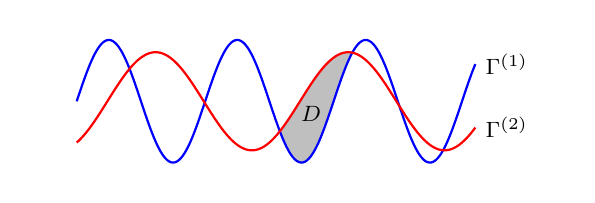
\begin{tikzpicture}
	\begin{axis}[xmax=8,axis lines=none,axis equal image=true]
		% two curves
		\addplot [blue,thick,smooth,samples=200,name path=gamma1,domain=0:6.5] {sin(3*\x r)} 
		         node [black,right] {\footnotesize$\Gamma^{(1)}$};
		\addplot [red,thick,smooth,samples=200,name path=gamma2,domain=0:6.5] {0.8*sin((2*\x-1) r)} 
		         node [black,right] {\footnotesize$\Gamma^{(2)}$};
		% fillbetween
		\addplot [white] fill between [of=gamma1 and gamma2, split, every segment no 3/.style={gray,opacity=0.5}];
		% notations
		\draw (axis cs:3.5,-0.2) node [right] {\footnotesize$D$};
	\end{axis}
	\end{tikzpicture}
\end{document}